\documentclass[9pt]{beamer}

\mode<presentation>
{
  \usetheme{HSE}
  \usecolortheme{default}
  \usefonttheme{serif}
  \setbeamertemplate{navigation symbols}{}
  \setbeamertemplate{caption}[numbered]
}

\usepackage{graphicx}
\usepackage{amsmath}
\usepackage{movie15}
\usepackage{varwidth}


\graphicspath{ {./images/} }

\DeclareMathOperator{\argmax}{argmax}

\title[]{
Clustering of Multidimensional Random Variables to Improve HMM Sequence Alignment Accuracy
}
\author[Denis Grachev]{Denis Grachev\\
\qquad\\\
Scientific supervisor:\\
PhD candidate, Timofey Prodanov}
\date{\today} % Date, can be changed to a custom date



%\usetheme{lucid}
\begin{document}
	\frame {
		\titlepage
	}

    \frame{
        \frametitle{Introduction to bioinformatics}
        \begin{itemize}
            \item The most useful biological data is DNA (genome) sequence.
            \item Each chromosome is represented as a string over alphabet $\{ A, C, G, T\}$.
            \item Most species are diploid $\Rightarrow$ each chromosome is paired.
            \item It is very large (human genome is 6.4 billion bp).
            \item Genomes of unrelated humans are $99.9\%$ similar. 
            \item Determine reference genome and identify difference for any individual.
        \end{itemize}
    }

    \frame {
        \frametitle{Reading genome}
        \begin{itemize}
            \item Read random peaces of genome (reads).
            \item Find similar peaces in reference genome (Alignment).
            \item Estimate difference (variant calling).
        \end{itemize}

        \begin{block}{Example}
            \begin{figure}
                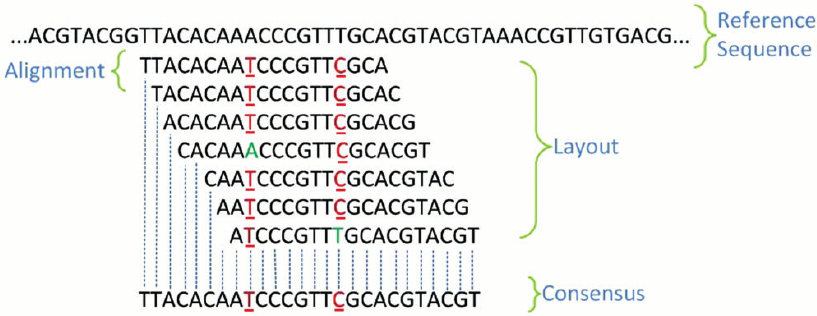
\includegraphics[scale=0.3]{aligned_reads}
                \caption{Reading genome example.}
            \end{figure}
        \end{block}
    }

    \frame {
        \frametitle{Alignment}
        Global alignment of two strings - way of representing 2 strings to spot similarities.
        \begin{block}{Idea}
            Assume that string $s_2$ was obtained from $s_1$ by applying 3 types of errors to it.
            \begin{itemize}
                \item Substitution. Replace one letter with another.
                \item Insertion. A letter was inserted to string.
                \item Delition. A letter was deleted from string.
            \end{itemize}
            Task is to find most likely sequence of errors for given $s_1$ and $s_2$.
        \end{block}
    }

    \frame{
        \frametitle{Alignment}
        \begin{block}{Example}
            Alignment of strings $s_1 = CABCAABA$ and $s_2 = ABADBBAD$ 
            over alphabet $\Sigma = \{ A, B, C, D\}$.
        
            \begin{center}
                Initial strings. \\
                \begin{tabular}{|| c | c c c c c c c c ||}
                 $s_1$ & C & A & B & C & A & A & B & A \\ 
                 $s_2$ & A & B & A & D & B & B & A &   \\    
                \end{tabular}
        
                \hfill \break 
        
                Aligned strings. \\
                \begin{tabular}{|| c | c c c c c c c c c ||}
                    $\hat{s}_1$ & C & A & B & C & - & A & A & B & A \\ 
                    $\hat{s}_2$ & - & A & B & - & A & D & B & B & A   
                \end{tabular}
        
            \end{center}
        \end{block}
    }

    \frame{
        \frametitle{Representing alignment as pair HMM}
        \begin{block}{Hidden states}
            \begin{itemize}
                \item M: Match or Mismatch.
                \item X: Insertion to $s_1$.
                \item Y: Insertion to $s_2$ (Delition).
            \end{itemize}   
        \end{block}

        \begin{block}{Observations}
            \begin{itemize}
                \item M: $\{ (x, y) \:|\: x, y \in \Sigma\}$.
                \item X: $\{ (x, -) \:|\: x \in \Sigma\}$.
                \item Y: $\{ (-, y) \:|\: y \in \Sigma\}$.
            \end{itemize}
            
        \end{block}
    }

    \frame{
        \frametitle{Representing alignment as HMM}
        \begin{block}{Example}
            Alignment of strings $s_1 = CABCAABA$ and $s_2 = ABADBBAD$ 
            over alphabet $\Sigma = \{ A, B, C, D\}$.
        
            \begin{center}
                Initial strings. \\
                \begin{tabular}{|| c | c c c c c c c c ||}
                 $s_1$ & C & A & B & C & A & A & B & A \\ 
                 $s_2$ & A & B & A & D & B & B & A &   \\    
                \end{tabular}
        
                \hfill \break 
        
                Aligned strings. \\
                \begin{tabular}{|| c | c c c c c c c c c ||}
                    $\hat{s}_1$ & C & A & B & C & - & A & A & B & A \\ 
                    $\hat{s}_2$ & - & A & B & - & A & D & B & B & A \\
                    O           & X & M & M & X & Y & M & M & M & M  
                \end{tabular}        
            \end{center}
        \end{block}
    }

    \frame{
        \frametitle{Representing alignment as HMM}
        \begin{block}{Scoring alignment}
            \begin{itemize}
                \item Based on HMM each alignment assigned a probability.
                \item Can find alignment with highest probability.
            \end{itemize}
        \end{block}

        \begin{block}{Picture}
            \begin{figure}
                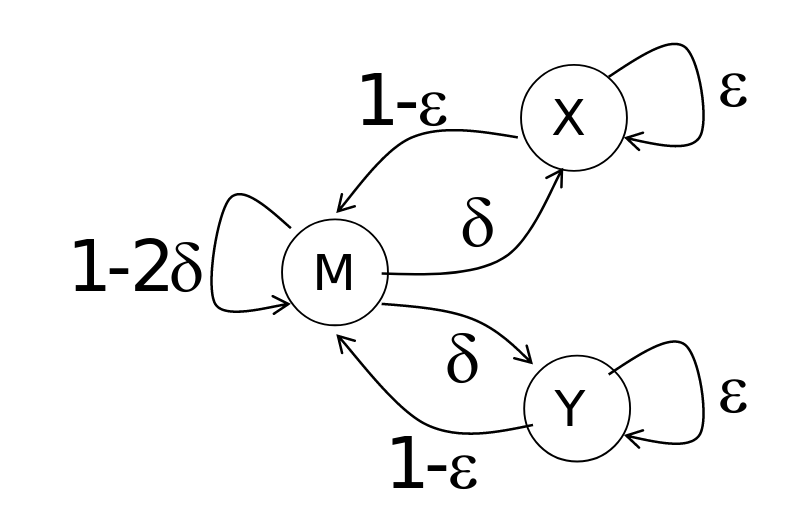
\includegraphics[scale=0.15]{Markov_chain.png}
                \caption{Picture of HMM}
            \end{figure}
        \end{block}
    }
    
    \frame{
        \frametitle{Variant calling}
        Longshot is a variant calling tool that uses same HMM to estimate difference.
        \begin{block}{Picture}
            \begin{figure}
                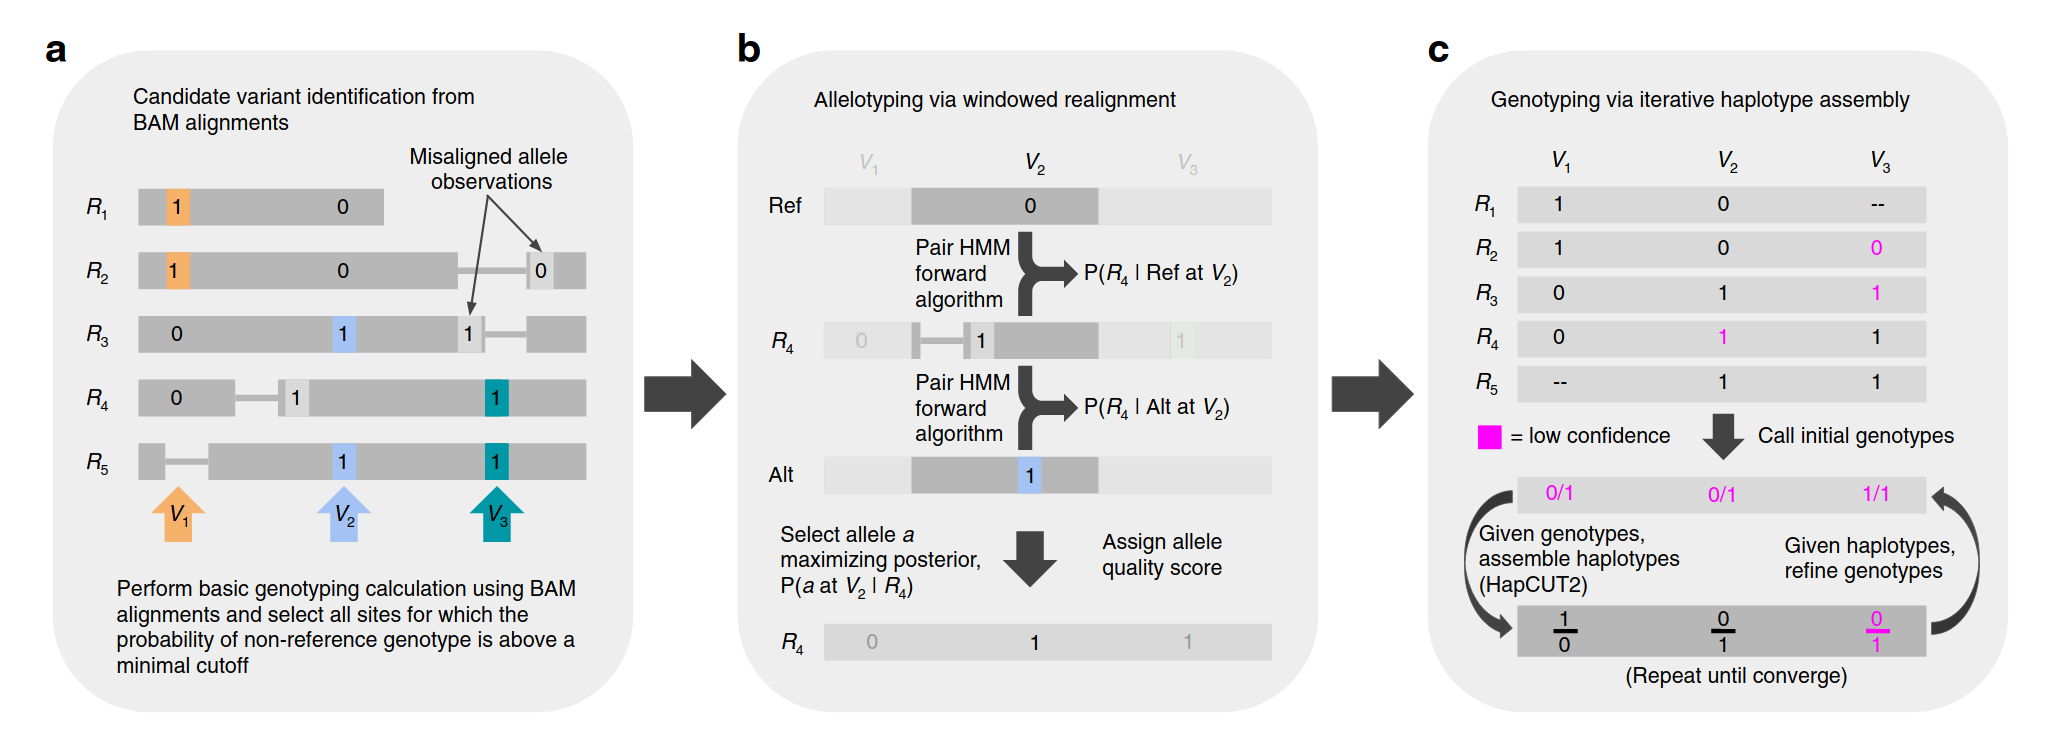
\includegraphics[scale=0.15]{longshot.png}
                \caption{Longshot algorithm}
            \end{figure}
        \end{block}
    }

    \frame{
        \frametitle{Improving accuracy}
        \begin{itemize}
            \item Different sequence technologies produce different read profiles.
            \item Reads obtained from different regions have different read profiles.
        \end{itemize}
        To improve accuracy of variant calling, we can use different transition probabilities for different read profiles.
        \begin{itemize}
            \item Develop an algorithm to group reads by their profile.
            \item Add such functionality to Longshot (in progress).
        \end{itemize}
        
    }
    

	\frame {
		\frametitle{Clustering}
        \begin{block}{Clustering}
		Given $ X = \{ x_i | x_i \in \mathbb{R}^d, i \in (1 \ldots n) \} $ and $l$ - number of clusters. \\ 
		Clustering is assigning each point to one cluster $C = \{ c_i | c_i \in (1 \ldots l), i \in (1 \ldots n) \} $. \\
		\end{block}

        \begin{block}{Example}
		for $\mathbb{R}^2$ and $l = 2$

        \begin{figure}
            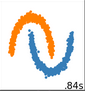
\includegraphics{example_clustering}
            \caption{Example of clustering}
        \end{figure}
        \end{block}
	}


    \frame {
        \frametitle{Algorithm}
        \begin{block}{Preprocess}
            \begin{enumerate}
                \item For each read calculate probability of each transitions. \\
                (MM, MI, MD $\ldots$)
                \item Each feateture is devided by standart deviation.
                \item PCA method is applied for resulting data.
            \end{enumerate}
        \end{block}

        \begin{figure}
            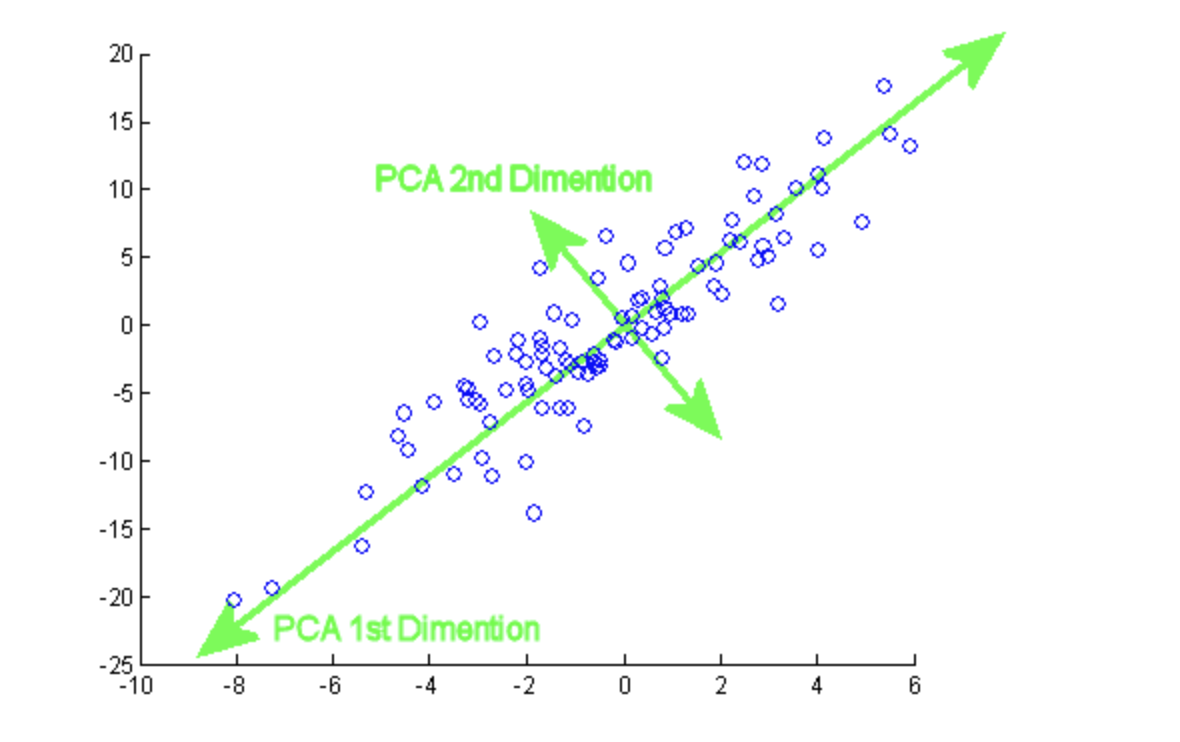
\includegraphics[scale=0.3]{pca.png}
            \caption{Example of PCA}
        \end{figure}
    }

    \frame{
        \frametitle{Algorithm}
    
        Assume that distribution in each cluster is multidimensional normal distribution.

        \begin{block}{Likelihood}
        $\Theta = \{ \theta_i | \theta_i \text{ - parameters of ith cluster} \}$ \\ 
        We can estimate parameters of each cluster based on $X$ and $C$. \\
        Denote ith class as $\omega_i$, then probability of $x$ belong to ith cluster is
        $$ p(x | \Theta) = p(x | \omega_i, \theta_i) P(\omega_i) $$ 

        \end{block}
    }

    \frame {
        \frametitle{Algorithm}
        Denote clusters as $ \chi_1 \ldots \chi_l $, than logarithm of probability for all points is of cluster is 

        \begin{align*}
            L_i &= \sum_{x \in \chi_i} \log(p(x| \omega_i, \theta_i)P(\omega_i)) \\
                &=  \sum_{x \in \chi_i} \log \left( 
                \frac{ \exp \left( \frac{-1}{2} (x - \mu_i)^T \Sigma_i^{-1} (x - \mu_i) \right) }
                {(2 \pi)^{d/2} |\Sigma_i| ^ {1/2}}
                \right) + n_i \log(P(\omega_i)) \\
                &= -\frac{1}{2} n_i d - \frac{n_i d}{2} \log(2 \pi) - \frac{n_i}{2} \log |\Sigma_i| + n_i \log \frac{n_i}{n}.
        \end{align*} 

        Where $\mu_i$ is mean value and $\Sigma_i$ - covariation of ith cluster.

        Overall likelihood is 
        $$ L = \sum_{i = 1}^l L_i$$ 
    }

    \frame {
        \frametitle{Algorithm}
        Move $\hat{x}$ from $\chi_i$ to $\chi_j$, then

        \begin{align*}
            \Delta L_i = &-\frac{1}{2} \log |\Sigma_i| + \frac{n_i - 1}{2} 
                \log \left(1 - \frac{(\hat{x} - \mu_i)^T \Sigma_i^{-1}(\hat{x} - \mu)}{n_i - 1} \right) + \\
                 &+ \log \frac{n_i}{n} - (n_i - 1)(\frac{d}{2} + 1) \log \frac{n_i - 1}{n_i}
        \end{align*}
        
        \begin{align*}
            \Delta L_j = &-\frac{1}{2} \log |\Sigma_j| - \frac{n_j + 1}{2} 
                \log \left(1 + \frac{(\hat{x} - \mu_j) \Sigma_j^{-1} (\hat{x} - \mu_j)}{n_j + 1}\right) + \\
                 &+ \log \frac{n_j}{n} + (n_j + 1)(\frac{d}{2} + 1) \log \frac{n_j + 1}{n_j}.
        \end{align*}

        \begin{align*}
            \Delta L &= \Delta L_i + \Delta L_j
        \end{align*}
    }

    \frame {
        \frametitle{Algorithm}
        \begin{block}{Idea}
            \begin{enumerate}
                \item Initialize clusters (randomly or using another algorithm)
                \item Iterate over all points
                \begin{enumerate}
                    \item Move point to a cluster, such that overall likelihood increases the most. (With most $\Delta L_j$)
                    \item Update clusters and their parameters.
                \end{enumerate}
                \item Repeat step 2 while it makes changes.
            \end{enumerate}
        \end{block}

        \begin{block}{Advantage}
            \begin{itemize}
                \item After every step overall likelihood increases.
                \item This implies that the cycle will end.
            \end{itemize}
        \end{block}

        \begin{block}{Problem}
            \begin{itemize}
                \item Updateting parameters after every step is very slow.
            \end{itemize}
        \end{block}
    }

    \begin{frame}
        \frametitle{Algorithm}
        \begin{block}{Fix 1}
            \begin{itemize}
                \item Update parameters every $k$ points.
                \item If overall likelihood decreased, revert changes.
            \end{itemize}
        \end{block}

        \begin{block}{Bad}
            \begin{itemize}
                \item Can stuck in a loop, transfering and reverting same points.
            \end{itemize}
        \end{block}

        \begin{block}{Fix 2}
            \begin{itemize}
                \item Pick points randomly and apply algorithm for them. Then repeat for other points.
            \end{itemize}
        \end{block}

    \end{frame}

    \frame {
        \frametitle{Algorithm}
        \begin{block}{Fixed}
            \begin{enumerate}
                \item Initialize clusters and estimate their parameters
                \item Divide $X$ into $p$ random disjoint groups $g_1 \ldots g_p$.
                \item Loop c from $1$ to $p$.
                \begin{enumerate}
                    \item Loop $x$ over $g_c$.
                    \begin{enumerate}
                        \item Let $x$ currently be in cluster $i$.
                        \item If $n_i <= 1$, then pass to next point.
                        \item Calculate $\delta_{j}=
                            \left\{\begin{array}{cc}
                            \Delta L_{j}, & j \neq i \\
                            \Delta L_{i}, & j=i
                            \end{array}\right. $
                        \item Transfer $x$ to $\argmax (\delta_j)$ cluster.
                    \end{enumerate} 
                    \item Update parameters.
                    \item If overall likelihood is not increased, revert changes.
                \end{enumerate}
                \item If any changes were made, repeat step 2.
            \end{enumerate}
        \end{block}
    }

    \frame{
        \frametitle{Algorithm}

        Example of work of the stepwise iterative maximum likelihood algorithm.

        \begin{varwidth}{\textwidth}
            \begin{figure}
                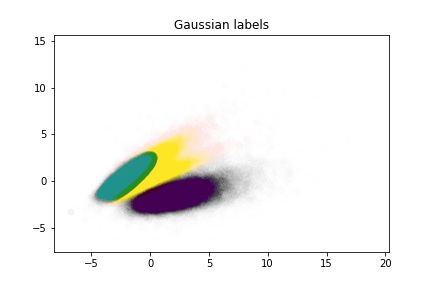
\includegraphics[width=0.55\textheight]{gaussian_generated_3.png}
                \caption{Initial clustering}
            \end{figure}
        \end{varwidth}
        \hfill
        \begin{varwidth}{\textwidth}
            \begin{figure}
                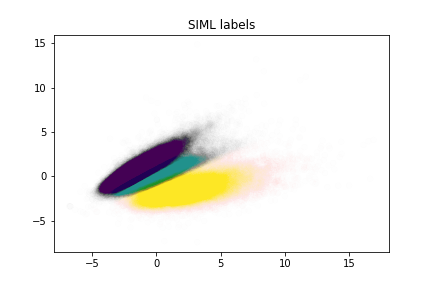
\includegraphics[width=0.55\textheight]{siml_generated_3.png}
                \caption{Obtained clustering}
            \end{figure}
        \end{varwidth}
    }

    \frame {
        \frametitle{In progress} {
            Implement proposed algorithm into Longshot. \\
            Cluster reads and use different transition probabilities for different clusters.\\
            Measure increase of accuracy. \\
            \hfill \break
            Thank admission committee.
        }
    }

\end{document}